\documentclass[12pt]{article}
\usepackage{anyfontsize}
\usepackage[a4paper, margin=2cm]{geometry}
\usepackage{polski}
\usepackage{tabto}
\usepackage{enumitem}
\usepackage{amsmath}
\usepackage{multirow}
\usepackage{multicol}
\usepackage{setspace}
\usepackage{tabularx}

\usepackage{graphicx}

\usepackage{chngcntr}
\counterwithin{figure}{section}
\counterwithin{table}{section}
\numberwithin{equation}{section}

\usepackage{hyperref}
\hypersetup{
    colorlinks = true,
    urlcolor=blue,
    linkcolor= black
}

\usepackage{graphicx}
\graphicspath{{../Img/}}

\usepackage{titlesec}
\titlelabel{\thetitle.\quad}
% \AddToHook{cmd/section/before}{\clearpage}

\usepackage[european, american currents, americanvoltages, RPvoltages, cute inductor]{circuitikz}
\usepackage{tikz}
\usetikzlibrary{shapes.geometric}
\ctikzset{
    logic ports=ieee,
    logic ports/scale=0.7,
}

% \renewcommand{\figurename}{Zdjęcie}


\title{Dokumentacja projektu\\ \textbf{FPGA Snake} {\small \\ z przedmiotu: Projektowanie Systemów Cyfrowych}}
\author{Łukasz Przystupa}
\date{\today}

\usepackage{titling}
\renewcommand\maketitlehooka{\null\mbox{}\vfill}
\renewcommand\maketitlehookd{\vfill\null}

\begin{document}
    \begin{titlepage}
        \maketitle
        \thispagestyle{empty}
        \begin{center}
            Opiekun projektu: Paweł Rajda
        \end{center}
    \end{titlepage}

    % \section*{Wstęp}
    \tab bla bla bla\newpage
    \section{Założenia projektowe}
    \tab Poniższy projekt zakłada stworzenie układu cyfrowego do gry w Snake.
    Gra będzie wyświetlana na monitorze wyposażonym w interface VGA.
    \subsection{Sterowanie}
        \tab Sterowanie odbywa się za pomocą dwóch przycisków,
        informujących głowę węża czy skręcić w prawo czy w lewo.
% 
        Dodatkowo należy wyróżnić dodatkowe dwa przyciski resetujące:
        \begin{itemize}
            \item [--] reset główny -- przycisk resetujący wszystkie procesy układu włącznie z procesami sterującymi VGA.
            \item [--] reset wewnętrzny -- restartuje wyłącznie stan gry.
        \end{itemize}

    \subsection{Wyświetlanie}
        \tab Gra toczy się na planszy składającej się z $40x30$ kratek,
        a wyświetlana w rozdzielczości $640x480$px.
        Do monitora podłączone są trzy sygnały kolorów dające w sumie 8 kolorów.

    \section{Opis funkcjonalny}
    % zdjęcie układu
    \begin{figure}[!ht]
        \centering
        \includegraphics[width=0.4\textwidth]{mimas.jpg}
        \renewcommand{\figurename}{Zdjęcie}
        \caption{Mimas -- płytka rozwojowa z układem Spartan 6}
        \label{fig:mimas}
    \end{figure}
    Na powyższym zdjęciu \ref{fig:mimas} przedstawiono zdjęcie płytki na której przeprowadzono testy.
    Głownym interfejsem komunikacyjnym są cztery przyciski podpisane prze producenta (licząc od dołu) SW1 do Sw4.
    \begin{enumerate}
        \item [SW4 -- ] reset wewnętrzny,
        \item [SW3 -- ] przycisk sterowania - skręć w lewo,
        \item [SW2 -- ] przycisk sterowania - skręć w prawo,
        \item [SW1 -- ] reset główny.
    \end{enumerate}
% 
    Nad przyciskami znajduje się pasek ośmiu ledów, które podczas gry wyświetlają animację sygnalizującą
    pracę układu.

    \subsection{Opis rozgrywki}
        \tab Zasady gry są proste gracz jest głową żarłocznego węża 
        i jego zadaniem jest tak kierować swoimi ruchami aby zjeść jak najwięcej czerwonych punktów.
        Jednocześnie starając się nie uderzyć w żadną ze ścian planszy oraz nie zjeść samego siebie.
        Dodatkowym utrudnieniem jest rozszerzanie się węża za każdym razem gdy zostanie zjedzony punkt.
        % Rozszerzanie to odbywa się poprzez ruc

        % \newpage
        Zachowanie węża przedstawia prosta maszyna stanów:
        \begin{figure}[!ht]
            \centering
            \begin{tikzpicture}
                \draw
                    ( 0,  0) node[draw, circle, align=center, minimum width = 2.5cm](start){Sprawdzenie\\kratki}
                    ( 4, -2) node[draw, circle, align=center, minimum width = 2.5cm](head){Ruch\\głowy}
                    ( 4, -6) node[draw, circle, align=center, minimum width = 2.5cm](capture){Zajęcie\\kratki}
                    ( 0, -8) node[draw, circle, align=center, minimum width = 2.5cm](tail){Ruch\\ogona}
                    (-4, -6) node[draw, circle, align=center, minimum width = 2.5cm](free){Zwolnienie\\kratki}
                    (-4, -2) node[draw, circle, align=center, minimum width = 2.5cm](wait){Czekaj}

                    ( 6,  0) node[draw, circle, align=center, minimum width = 1cm](reset){Reset}
                ;
                \draw [thick, -Straight Barb] (start)    edge[bend left] (head);
                \draw [thick, -Straight Barb] (head)     edge[bend left] (capture);
                \draw [thick, -Straight Barb] (capture)  edge[bend left] (tail);
                \draw [thick, -Straight Barb] (capture)  edge[bend left] node[rotate = -25, above]{Dodaj punkt} (wait);
                \draw [thick, -Straight Barb] (tail)     edge[bend left] (free);
                \draw [thick, -Straight Barb] (free)     edge[bend left] (wait);
                \draw [thick, -Straight Barb] (wait)     edge[bend left] (start);
                % \draw [thick, -Straight Barb] (wait)     edge[loop left] (wait);
                \draw [thick, -Straight Barb] (reset)     edge[bend right] (head);
                \draw [thick, -Straight Barb] (start)    edge[bend left] node[rotate = 90, above]{Zniszcz się} (tail);
                \draw [thick, -Straight Barb] (free)     edge[bend left] node[rotate =-25, above]{Zniszcz się} (tail);
            \end{tikzpicture}

            \renewcommand{\figurename}{Schemat}
            \caption{Algorytm działania węża}
            \label{schematic:snake}
        \end{figure}
        
        Powyższy opis (schemat \ref*{schematic:snake}) należy rozbudowa o kilka słów komentarza,
        \begin{enumerate}
            \item Sprawdzenie kratki, sprawdza stan sprawdza nie tylko czy nie wystąpiła kolizja, ale także czy został zdobyty punkt. 
            Na tej podstawie wystawiany jest specjalny, odpowiadający za dodanie punkt lub za samozniszczenie.
            \item W momencie ruchu głowy na rejestrze FIFO, zapisywany jest kierunek ruchu, który po odczytaniu służy ogonowi za pamięć w jakim kierunku ma się poruszyć.
            \item W trakcie samozniszczenia, powstaje pętla między, która traw do restartu procesu. Jednak ogon nie porusza się w nieskończoność a jedynie do momentu opróżnienia rejestru FIFO.
            \item Zajęcie/zwolnienie kratki w rzeczywistości odbywa się w tym samym takcie zegarowym co ruch głowy/ogona, jednak ze względu na czytelność te operacje zostały wyróżnione.
        \end{enumerate}

        
    \subsection{Generowanie punktów}
        \tab Miejsce pojawienia się punktu na mapie jest 16 pseudolosową liczbą, z której górna połówka odpowiada za współrzędną $y$, natomiast dolna za współrzędną $x$.
        Tak wygenerowane współrzędne następnie są porównywane z mapą i jeśli kratka o tych współrzędnych jest wolna, pojawia się punkt.

    \subsection{Przegrana}
        \tab Gracz kończy rozgrywkę w momencie zderzenia z samym sobą lub ze ścianą.
        W chwili zderzenia, wyzwolone zostają sygnały sterujące animacją destrukcji
        a wynik gracza zostaje zatrzaśnięty oraz wyświetlony na planszy.



    \section{VGA}
    \tab Jak widać na zdjęciu \ref{fig:mimas}, płytka \underline{nie} jest wyposażona we wbudowane złącze VGA,
    wymagane więc dołożenia zewnętrznego złącza, oraz rezystorów szeregowych, 
    pozwalających na spełnienie standardu napięć VGA. Poniżej przedstawiono schemat połączeń jakie należy wykonać.

    \begin{figure}[!ht]
        \centering
        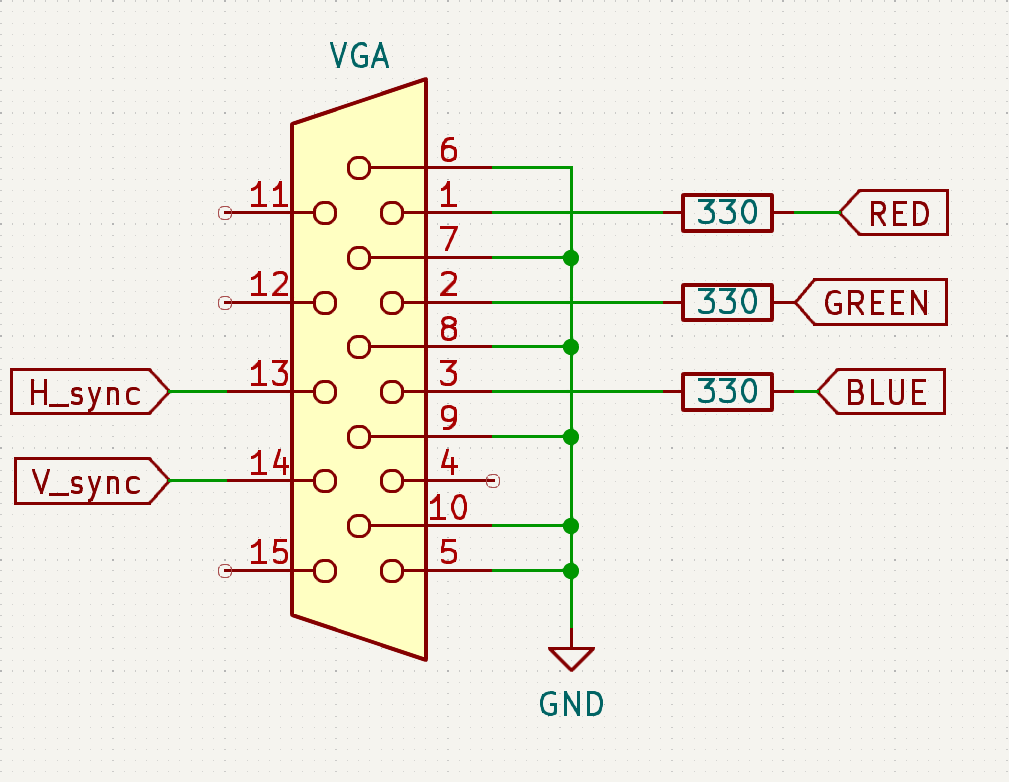
\includegraphics[width = 0.7\textwidth]{VGA.png}
        \renewcommand{\figurename}{Schemat}
        \caption{Złącze VGA}
    \end{figure}

    Zgodnie ze standardem, zakres napięć ograniczony jest od dołu: $0V$ (pełna czerń) do maksymalnie: $0.7V$ (pełen kolor).
    Dodatkowo, impedancja wejściowa oscyluje w okolicy $75\Omega$. 
    A więc dołączenie sygnału o napięciu $3.3V$ przez rezystor o wartości $\ge 280\Omega$ pozwala dostosować progi napięciowe do standardu, zgodnie ze wzorem (\ref{equ:voltage_devider}):
    
    \begin{equation}
        V_o = V_i \cdot \frac{75\Omega}{75\Omega + R_{\text{color}}}
        \label{equ:voltage_devider}
    \end{equation}
    % W projekcie zostały wykorzystane rezystory z szeregu E24, o wartości większej od przyjętej minimalnej - $330\Omega$

    Poniżej przedstawiono schemat blokowy modułu odpowiadającego za synchronizację sygnałów VGA:
    \begin{figure}[!ht]
        \centering
        \begin{circuitikz}
            \draw
                (0, 0) node [draw, align=center, minimum width = 4cm] (H_cnt){Licznik horyzontalny\\$mod\ 800$}
                (6, 0) node [draw, align=center, minimum width = 4cm] (V_cnt){Licznik wertykalny  \\$mod\ 525$}
                (H_cnt.west) to[short, i<=\ , -o] (-3, 0) node[left]{25MHz}
                (H_cnt.east) to[short, i>=Reset] (V_cnt.west)

                (7, -1.75) node[and port, number inputs=3, anchor = out](color_en){}

                (-3, -2) coordinate(color) node[left]{Color}
                (color) to[short, o-, tmultiwire] ++ (2, 0) -- (color_en.in 3)
                (color_en.out) to[short, -o, tmultiwire] ++ (1.5, 0) node[right]{RGB}
                (H_cnt.south) ++ ( 0, 0) -- (0, -1.75) to[short, i=Draw Enable] (color_en.in 2)
                (V_cnt.south) ++ (-1, 0) to[short, i=Draw Enable] ++ (0,-0.95) -- (color_en.in 1)

                (H_cnt.south) ++ ( 1, 0) |- (8.5,-1.25) to[short, -o] ++ (0, 0) node[right]{$H_{sync}$}
                (V_cnt.south) ++ ( 1, 0) |- (8.5,-0.75)    to[short, -o] ++ (0, 0) node[right]{$V_{sync}$}

            ;
        \end{circuitikz}
        \renewcommand{\figurename}{Schemat}
        \caption{Schemat blokowy VGA}
        \label{schematic:VGA}
    \end{figure}




    \section{Opis całego układu}
    \subsection{Schemat blokowy}
        \begin{figure}[!ht]
            \centering
            \begin{circuitikz}
                \draw
                    (0,   0) node[draw, minimum width = 4cm, minimum height = 2cm](clk){Podział zegarów}
                    (6,   0) node[draw, minimum width = 4cm, minimum height = 2cm](led){Animacja LED}
                    (8,  -3) node[draw, minimum width = 4cm, minimum height = 2cm](vga){VGA}
                    (4,  -7) node[draw, minimum width = 4cm, minimum height = 2cm](map){Kontroler mapy}
                    (12, -7) node[draw, minimum width = 4cm, minimum height = 2cm](score){Wyświetlanie punktów}
                    (7, -10) node[draw, minimum width = 4cm, minimum height = 2cm](snake){Wąż}
                    (0, -7) node[draw, minimum width = 2cm, minimum height = 2cm, align=center](point){Generator\\punkow}
                    (4, -14) node[draw, minimum width = 4cm, minimum height = 2cm, align=center](mem)  {Pamięć pozycji  \\ (ROM)}
                    (10,-14) node[draw, minimum width = 4cm, minimum height = 2cm, align=center](fifo) {Pamięć kierunku \\ (FIFO)}
                    (10.5, -9.5)node[and port, anchor=in 1, rotate = 90](score_en){}

                    (led.east) to[short, -o, i=\ ] ++ (4, 0) node[right]{Leds}
                    (0, -10) coordinate(turn) node[left, align=center]{Turn\\left/right} (turn) to[short, i=\ , o-] (snake.west)

                    (clk.south) to[short] ++ (0, -2) to[short, i= 25MHz] (vga.west)
                    (clk.east) to[short, i=8Hz] (led.west)
                    % (clk.south) to[short] ++ (0, -6) to[short, i=100MHz, *-] (map.west)
                    % (clk.south) to[short] ++ (0, -6) to[short, i=100MHz] ++ (0, -2)

                    (map.south) to[short, i=XY] ++ (0, -1.25) -- ++ (1, 0)

                    (point.east) to[short, i=XY] (map.west)
                    (snake.north) ++ (-1.5, 0) to[short, i_=Draw] ++ (0, 1) 
                    (snake.north) ++ (0, 0) to[short] ++ (0, 1.5) to[short, i<_=Push] ++(-1, 0)
                    (snake.north) ++ (1, 0) to[short] ++ (0, 2.5) to[short, i<_=Destroy] ++(-2, 0)
                    (snake.east) ++ (0, 0.5) to[short, i>_=Destroy] (score_en.in 1)
                    (fifo.north) ++ (0.9, 0) to[short, i_=Score] (score_en.in 2)

                    (vga) to[short, -*, i=XY] ++ (0, -2.5) coordinate(xy)
                    (xy) -| (score.north)
                    (xy) -| (map.north)

                    (score.north) ++ (1, 0) to[short] ++ (0, 1) to[short, i_=Score] ++ (-3.5, 0) --++(0, 1)
                    (map.north) ++ (-1, 0) to[short] ++ (0, 1) to[short, i=Color] ++ (3.5, 0) --++(0, 1)

                    (snake.west) ++ (0, -0.75) to[short] ++ (-1, 0) coordinate(xy) to[short, i_=FILL] ++ (0, -2.25)
                    % (xy) to[short, *-, i=\ ] ++(0, 2)
                    (snake.south) ++ (-1.75, 0) to[short, i_=RW] ++ (0, -2)
                    (mem.east) -- ++ (0.5, 0) to[short, l=XY] ++ (0, 3)

                    (fifo.west)-- ++ (-.5, 0) to[short, a=Dir] ++ (0, 3)
                    (snake.east) ++ (0, -.5) --++ (0.5, 0) to[short, i=RW] ++ (0, -2.5)


                    (vga.east) ++ (0, 0.5) to[short, i=\ , -o] ++ (2, 0) node[right]{$H_{sync}$}
                    (vga.east) ++ (0, 0.0) to[short, i=\ , -o] ++ (2, 0) node[right]{$V_{sync}$}
                    (vga.east) ++ (0,-0.5) to[short, i=\ , -o] ++ (2, 0) node[right]{$RGB$}
                ;
            \end{circuitikz}
            \renewcommand{\figurename}{Schemat}
            \caption{Schemat blokowy całej gry}
            \label{schematic:all_game}
        \end{figure}

        Na schemacie \ref{schematic:all_game}, przedstawiono uproszczony widok całego układu.
        Do każdego z elementów do którego nie został dociągnięty żaden sygnał zegarowy domyślnie jest podłączony zegar główny $100MHz$.
        Dodatkowo pamięci (pamięć pozycji oraz pamięć kierunku), zostały stworzone jako IP Core.

        % \subsubsection{Opis wyprowadzeń}
        \begin{table}[!ht]
            \centering
            \begin{tabular}{c | c}
                Wejścia & Wyjścia\\\hline
                & Leds[8]\\ 
                Turn left/right[2]& $H_{sync}$, $V_{sync}$ \\
                & $RGB$[3]

            \end{tabular}
            \caption{Opis wyprowadzeń}
        \end{table}
    % \subsection{Opis słowny}
    \subsection{Tabela wyprowadzeń}
    \begin{table}[!ht]
        \begin{tabularx}{\textwidth}{|l|c|c|X|}\hline
            Nr. & Nazwa & kierunek & Opis\\\hline
            \hline
            \multicolumn{4}{|c|}{\textbf{Top}}\\\hline
            1. & CLK                & in & wejście zegara modułu $100MHz$\\\hline
            2. & Reset              & in & wejście głównego resetu -- przycisk pop prawej stronie modułu\\\hline
            3. & SoftReset          & in & wejście resetu gry  -- przycisk pop lewej  stronie modułu\\\hline
            4. & LED $\#8$          & out & wyprowadzenia do diod LED\\\hline
            5. & H\_sync            & out & wyjście synchronizacji poziomej\\\hline
            6. & V\_sync            & out & wyjście synchronizacji pionowej\\\hline
            7. & RGB $\#3$          & out & wyjście koloru\\\hline
            8. & leftRight $\#2$    & in & wejścia do przycisków sterujących\\\hline
            \hline
            \multicolumn{4}{|c|}{\textbf{Top $\rightarrow$ VGA}}\\\hline
            1. & CLK    & in  & wejście zegara taktującego VGA $25MHz$\\\hline
            2. & Reset  & in  & wejście resetu - połączone bezpośrednio do resetu głównego\\\hline
            3. & V\_sync& out & wyjście synchronizacji poziomej generowanej w układzie \\\hline
            4. & H\_sync& out & wyjście synchronizacji pionowej generowanej w układzie \\\hline
            5. & RGB   $\#3$& out & wyjście koloru, będące iloczynem logicznym wejścia \textit{Color} i zezwolenia na wyświetlanie\\\hline
            6. & Color $\#3$& in  & wejście koloru, podawane przez mapę\\\hline
            7. & x $\#10$& out & wyjście wewnątrz układowe aktualnie wyświetlanej współrzędnej $x$ \\\hline
            8. & y $\#9$& out & wyjście wewnątrz układowe aktualnie wyświetlanej współrzędnej $y$ \\\hline
            \hline
            \multicolumn{4}{|c|}{\textbf{Top $\rightarrow$ Map\_controler}}\\\hline
            1. & CLK         & in  & wejście głównego zegara $100MHz$ \\\hline
            2. & Reset       & in  & logiczny iloczyn zegara głównego i zegara gry\\\hline
            3. & x $\#7$     & in  & główna współrzędna wyświetlanej kratki\\\hline
            4. & sub\_x $\#4$& in  & $\frac{1}{16}$ współrzędnej $x$ do wyświetlania sprite'ów (nie używane)\\\hline
            5. & y $\#6$     & in  & główna współrzędna wyświetlanej kratki\\\hline
            6. & sub\_y $\#4$& in  & $\frac{1}{16}$ współrzędnej $y$ do wyświetlania sprite'ów (nie używane)\\\hline
            7. & color $\#3$ & out & wyjście wyświetlanego koloru w odpowiedzi na podane współrzędne\\\hline
            8. & leftRight$\#3$& in  & wejście sterujące wężem \\\hline
            \hline
            \multicolumn{4}{|c|}{\textbf{Top $\rightarrow$ Map\_controler $\rightarrow$ Snake}}\\\hline
            1. & CLK         & in  & wejście głównego \\\hline
            2. & Reset       & in  & logiczny iloczyn zegara głównego i zegara gry\\\hline
            3. & x $\#7$     & in  & główna współrzędna wyświetlanej kratki\\\hline
            4. & y $\#6$     & in  & główna współrzędna wyświetlanej kratki\\\hline
            8. & leftRight$\#3$& in  & wejście sterujące wężem \\\hline
            6. & Part $\#3$  & out & wyjście informujące o tym jaka część węża ma być wyświetlana \\\hline
            7. & push        & in  & wejście logiki odpowiadającej za rozszerzenie się węża po zjedzeniu punktu \\\hline
            8. & max\_size$\#13$& out & wyjście wyniku (długości węża) w czasie gry wartość jest równa 0 \\\hline
        \end{tabularx}
    \end{table}
        \newpage
    \begin{table}[!ht]
        \begin{tabularx}{\textwidth}{|l|c|c|X|}\hline
            \multicolumn{4}{|c|}{\textbf{Top $\rightarrow$ Map\_controler $\rightarrow$ Apple\_generator}}\\\hline
            1. & CLK         & in  & wejście głównego \\\hline
            2. & Reset       & in  & logiczny iloczyn zegara głównego i zegara gry\\\hline
            3. & CanDraw     & in  & wejście blokujące w przypadku, gdy dana kratka jest zajęta\\\hline
            3. & x $\#7$     & in  & główna współrzędna wyświetlanej kratki\\\hline
            4. & y $\#6$     & in  & główna współrzędna wyświetlanej kratki\\\hline
            5. & apple       & out & wyjście koloru punkt, w momencie gdy VGA, zapyta o współrzędną $xy$, sygnał ustawiana jest na wysoki\\\hline
            6. & done        & out & wyjście informujące o tym, że punkt jest generowany i ma ustawione współrzędne\\\hline
            \hline
            \multicolumn{4}{|c|}{\textbf{Top $\rightarrow$ Map\_controler $\rightarrow$ Print\_digit}}\\\hline
            1. & CLK         & in  & wejście głównego \\\hline
            2. & Reset       & in  & logiczny iloczyn zegara głównego i zegara gry\\\hline
            3. & x $\#7$     & in  & główna współrzędna wyświetlanej kratki\\\hline
            4. & y $\#6$     & in  & główna współrzędna wyświetlanej kratki\\\hline
            5. & Data $\#13$ & in  & wejście wyniku, podawane w momencie przegranej\\\hline
            6. & Draw        & out & wyjście koloru, w momencie gdy VGA poda współrzędne danego punktu, sygnał draw wystawi informację czy kratka ma być zapełniona czy nie\\\hline
        \end{tabularx}
        \caption{Zawartość modułu}
    \end{table}
    \subsection{Dodatkowe pliki}
    \subsection{Pamięci węża i mapy}
        \tab Wąż wyposażony jest w dwie pamięci:
        \begin{enumerate}
            \item 1 bitowa pamięć RAM -- o wymiarach równych wymiarom mapy, w której przechowywane są poszczególne segmenty węża,
            \item 2 bitowy rejestr FIFO -- o głębokości równej iloczynowi wymiarów mapy ($\text{deeph} = x\cdot y$).
        \end{enumerate}
        Oba te moduły zostały wygenerowane przez środowisko jako IP Core.
    \subsubsection{Generator pseudolosowy}
        \tab Generator liczb pseudolosowych zastosowany w projekcie to prosty 16 bitowy scrambler.
        Rozwiązania równań zostały wzięte z dokumentu PDF, przygotowanego przez Xilinx'a.
        Rozdzielczość scramblera pozwala na dość dokładną emulację wartości losowej.

        16 bitowa rozdzielczość, pozwala na pokrycie dużo większej przestrzeni niż cała mapa.
        Dlatego, wartości odczytywane z scramblera, zostały podzielone w taki sposób, że:
        \begin{align}
            \text{starsza połówka}\ modulo(\text{szerokość mapy}) \Rightarrow x \\
            \text{młodsza połówka}\ modulo(\text{wysokość mapy}) \Rightarrow y 
        \end{align}
    \newpage
    \subsubsection{Wyświetlanie wyniku}
        \tab Wynik odczytywany odczytywany jest z licznika wbudowanego w rejestr FIFO
        i przekazywany do modułów zamieniających Naturalny Kod Binarny $(NKB)$ w kod $BCD_{10}$, zgodnie z wzorem:
        \begin{align}
            &\text{Ones} &=& &\frac{Data}{1}\ modulo(10) \\
            &\text{Tens} &=& &\frac{Data}{10}\ modulo(10) \\
            &\text{Hundreds} &=& &\frac{Data}{100}\ modulo(10) \\
            &\text{Thousands} &=& &\frac{Data}{1000}\ modulo(10)
        \end{align}

        Następnie z uprzednio zaprogramowanej pamięci ROM (również stworzonej jako IP Core),
        odczytywane są wartości, poszczególnych kratek w zależności dla każdej liczby, a ich wartość (kolor wyświetlany) przekazywana jest do układu sterującego \textit{VGA}.
    % \subsubsection{}


    \section{Podsumowanie}
    \tab Powyższy projekt był bardzo przyjemnym doświadczeniem, 
    pokazującym olbrzymią przewagę układów FPGA nad mikroprocesorami
    w sytuacjach, kiedy trzeba generować przebiegi o stałych parametrach,
    niezależnie od pozostałych operacji wykonywanych przez układ.
    Przykładowo generowanie sygnałów VGA, które na mikrokontlorerze jest w większości niemożliwe (lub bardzo trudne) a na bramkach logicznych jest to bajecznie proste.\\
    Z drugiej strony projekt pokazał też wady programowalnych układów logicznych i ich słabości w wykonywaniu
    wydawałoby się prostych (ale bardzo wyspecjalizowanych) operacji, takich jak dodawanie czy liczenie reszty z dzielenia.

    \subsection*{Wniosek końcowy}
        \tab Układy FPGA, są niezwykle wygodną formą budowania dużych 
        i skomplikowanych układów logicznych. 
        Jednak, współpraca z zewnętrznymi wyspecjalizowanymi układami 
        (t.j.: m.in.: pamięci RAM, mikroprocesory czy układy ALU) 
        jest niezbędna do optymalizacji zużycia zasobów.


\end{document}